\chapter{Введение}

При оценке драгоценного камня одним из важнейших факторов является качество огранки. В связи с этим, чтобы уменьшить влияние текущих дефектов на стоимость камня, важной задачей является идентификация примитивов, аппроксимирующих различные части камня. \vspace{0.5cm}

В данном документе речь пойдет о \textit{рундисте}, части многогранника, аппроксимируемой цилиндрической поверхностью.

\begin{figure}[h!]
\center{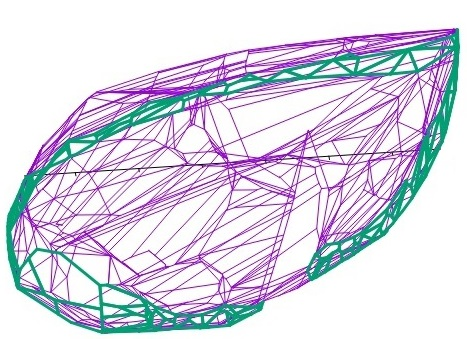
\includegraphics[scale=0.9]{Rundist.jpg}}
\end{figure}\newpage

\begin{center}
	\textbf{ \Large{Краткий обзор глав.}}
\end{center}

\noindent \textbf{ \large{Глава "1.Введение".}} 

В введении поясняется, с какой целью создан данный документ.\vspace{1cm}

\noindent\textbf{ \large{Глава "2.Цилиндрическая поверхность".}} 

В этой главе будут даны необходимые общие понятия о цилиндрических поверхностях.\vspace{1cm}

\noindent \textbf{ \large{Глава "3.Числовые характеристики".}} 

Раздел описывает статистики, рассчитываемые для цилиндрических поверхностей.\vspace{1cm}

\noindent \textbf{ \large{Глава "4.Рундист".}}

Дается определение рундиста на основе вычисленных статистик.\newpage